
\documentclass{article}
\usepackage[utf8]{inputenc}

% set font encoding for PDFLaTeX or XeLaTeX
\usepackage{ifxetex}
\ifxetex
  \usepackage{fontspec}
\else
  \usepackage[T1]{fontenc}
  \usepackage[utf8]{inputenc}
  \usepackage{lmodern}
\fi

% used in maketitle
\title{Reporte de Actividad 1}
\author{Roberto Benard Orci}
\date{30/01/2018}
% Enable SageTeX to run SageMath code right inside this LaTeX file.
% documentation: http://mirrors.ctan.org/macros/latex/contrib/sagetex/sagetexpackage.pdf
% \usepackage{sagetex}

\begin{document}
\maketitle

\section{Introducción}

El propósito de esta actividad es familiarizarse con la manera de hacer un reporte en Latex (usando imágenes de creative commons, citas estilo APA, etc). En esta actividad haremos un resumen del artículo de wikipedia sobre la atmósfera terrestre, en el cual usaremos la estructura que probablemente usaremos para otros reportes. Básicamente, esta actividad será nuestra guía para las siguientes actividades.

\section{Atmósfera Terrestre}

La atmósfera de la Tierra es la capa de gases, principalmente aire, que rodea al planeta Tierra y es retenida por la gravedad de la Tierra. La cantidad de aire y la presión atmosférica varían en las diferentes capas, el aire adecuado para su uso en la fotosíntesis por plantas terrestres y la respiración de animales terrestres se encuentra solo en la troposfera terrestre y en atmósferas artificiales.

\vspace{0.5cm}

\begin{center}
	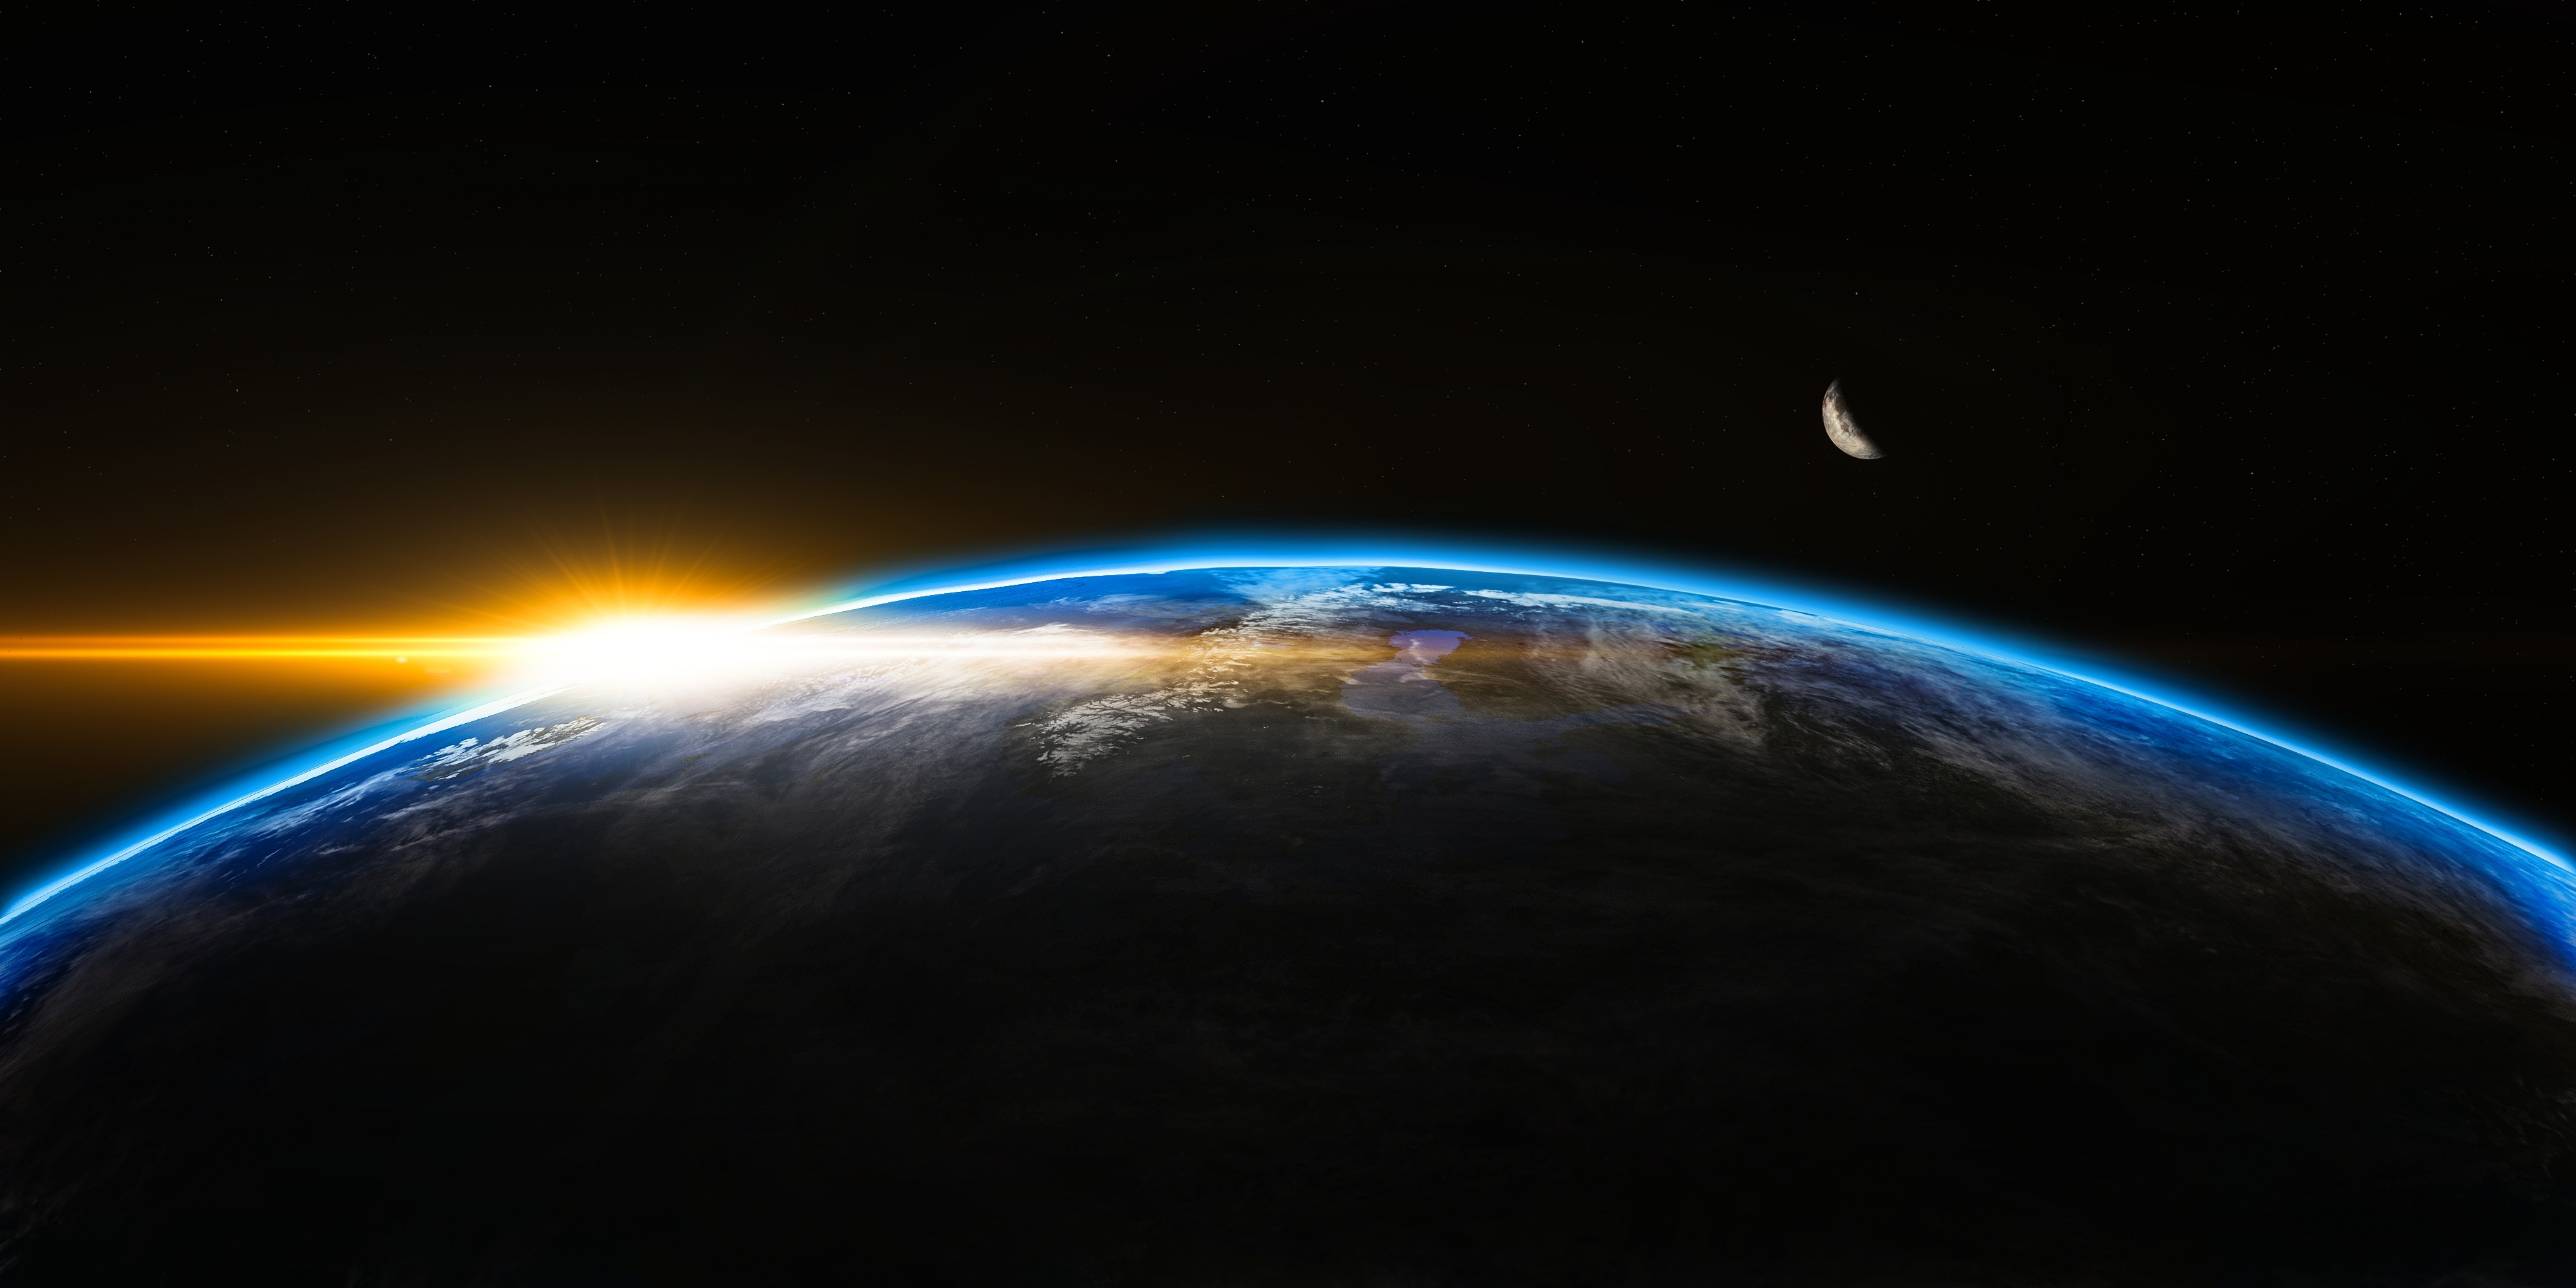
\includegraphics[width=\linewidth]{Atmosphere.jpeg}
    Atmósfera terrestre
\end{center}

\subsection{Composición}

Los tres componentes principales de la atmósfera son nitrógeno, oxígeno y argón (los cuales también son los tres componentes principales del aire). Asimismo, ésta contiene vapor de agua, la concentración de éste varía desde aproximadamente 10 ppm en las partes más frías de la atmósfera hasta 5\% de volumen en masas de aire caliente y húmedo. Los gases restantes a menudo se denominan gases traza, entre los cuales se encuentran los gases de efecto invernadero, principalmente dióxido de carbono, metano, óxido nitroso y ozono.

\subsection{Estructura de la Atmósfera}

La atmósfera de la Tierra se puede dividir en cinco capas principales: troposfera, estratosfera, mesosfera, termosfera y exosfera (de menor a mayor).
la densidad y presión atmosférica disminuyen conforme aumenta la altitud. La temperatura de la atmósfera terrestre varía con la altitud, la relación entre la altitud y la temperatura es distinta dependiendo de la capa atmosférica.

También existen capas secundarias dentro de las cinco capas principales. Estas están clasificadas por cierta característica que las distingue del resto de la capa principal (como una mayor concentración de cierto tipo de gas, o la ocurrencia de algún fenómeno atmosférico).

\vspace{0.5cm}

\begin{center}
	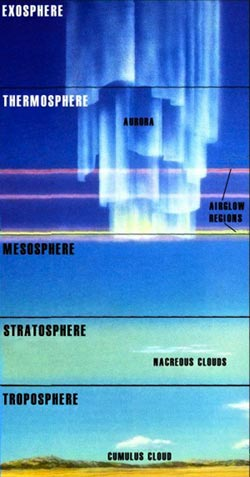
\includegraphics[width=4cm]{Earth_s_atmosphere.jpg}
    
    Estructura de la Atmósfera
\end{center}

\subsection{Propiedades físicas}

La mayoría de las propiedades tienen un aumento, o disminuye, con una relación constante/exponencial. Por ejemplo, la densidad del aire y la presión atmosférica disminuyen con el aumento de altitud, mientras que la temperatura disminuye conforme aumenta la amplitud, pero tiene ciertos lapsos en los que se estabiliza o incrementa por la interacción de la radiación con los gases en los distintos niveles de la atmósfera. Otra propiedad es la velocadad del sonido, la cual es directamente proporcional a la temperatura.

\subsection{Propiedades ópticas}

La atmósfera posee ciertas propiedades ópticas muy interesantes. Una de ellas es la dispersión de Rayleigh, que es la dispersión de la luz visible o cualquier otra radiación electromagnética por partículas cuyo tamaño es mucho menor que la longitud de onda de los fotones dispersados. Ocurre cuando la luz viaja por sólidos y fluidos transparentes, pero se ve con mayor frecuencia en los gases. La dispersión de Rayleigh de la luz solar en la atmósfera es la principal razón de que el cielo se vea azul.

\vspace{0.5cm}


Otros fenómenos son la absorción y la emisión de luz. En la absorción los gases absorben la radiación solar, mientras que, en la emisión, ciertos objetos han absorbido tanta radiación que se calientan hasta el punto en que terminan emitiendo radiación.

\vspace{0.5cm}


También está el índice de refracción de los gases. Las variaciones en el índice de refracción pueden conducir a la flexión de los rayos de luz en trayectos ópticos largos. Un ejemplo es que los observadores a bordo de barcos pueden ver otras embarcaciones justo sobre el horizonte porque la luz se refracta en la misma dirección que la curvatura de la superficie de la Tierra.
El índice de refracción depende de la temperatura.

\subsection{Circulación}

La circulación atmosférica es el movimiento de aire a gran escala a través de la troposfera, y la manera en la que se distribuye el calor alrededor de la Tierra. La configuración a gran escala de la circulación atmosférica varía de un año a otro, pero la estructura fundamental permanece básicamente constante porque está determinada por la velocidad de rotación de la Tierra y la diferencia en la radiación solar entre el ecuador y los polos.

\vspace{0.5cm}

\begin{center}
	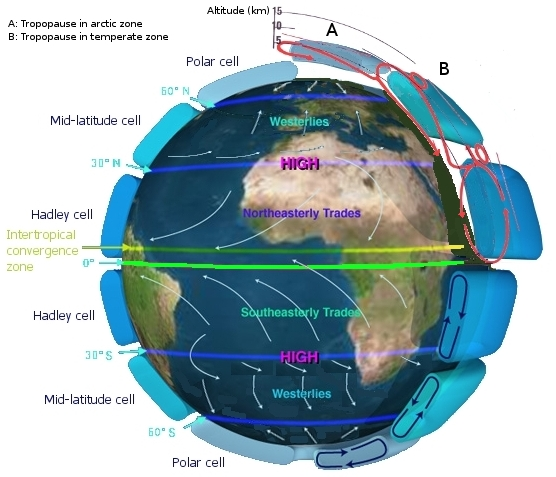
\includegraphics[width=10cm]{Earth_Global_Circulation.jpg}
    
    Circulación de aire en la Atmósfera
\end{center}

\section{Bilbiografía}

\begin{verbatim}
Atmósfera terrestre. (n.d.). Retrieved January 29, 2018, from
https://es.wikipedia.org/wiki/Atm\%C3\%B3sfera_terrestre#Capas_de_la_atm
\%C3\%B3sfera_terrestre_y_la_temperatura
\end{verbatim}

%https://es.wikipedia.org/wiki/Atm%C3%B3sfera_terrestre#Capas_de_la_atm%C3%B3sfera_terrestre_y_la_temperatura

\begin{verbatim}
Atmosphere of Earth. (2018, January 28). Retrieved January 29, 2018, from 
https://en.wikipedia.org/wiki/Atmosphere_of_Earth
\end{verbatim}

%https://en.wikipedia.org/wiki/Atmosphere_of_Earth#Physical_properties

\begin{verbatim}
Dispersión de Rayleigh. (2018, January 03). Retrieved January 29, 2018, from 
https://es.wikipedia.org/wiki/Dispersi%C3%B3n_de_Rayleigh
\end{verbatim}

%https://es.wikipedia.org/wiki/Dispersi%C3%B3n_de_Rayleigh

\begin{verbatim}
Wikimedia, 14/02/2010, Earth's Atmosphere, from
https://commons.wikimedia.org/wiki/File:Earth%27s_atmosphere.jpg
\end{verbatim}

\begin{verbatim}
qimono, Free stock photo of 3d, above, atmosphere, from
https://pixabay.com/en/sunrise-space-outer-globe-world-1765027/
\end{verbatim}

\begin{verbatim}
Wikimedia, 29/10/2009, File:Earth Global Circulation, from
https://commons.wikimedia.org/wiki/File:Earth_Global_Circulation.jpg
\end{verbatim}

\vspace{0.2cm}

\section{Apéndice}

1.	¿Qué fue lo que más te llamó la atención de esta actividad?

Tener que subir el reporte a la plataforma de github, ya que jamás la había usado, ni siquiera había oído hablar de ella.

\vspace{0.3cm}


2.	¿Qué fue lo que se te hizo menos interesante?

Trabajar con Latex. Solo había usado Latex una vez en Fortran, pero fuera de eso, Latex es relativamente nuevo para mí.  

\vspace{0.3cm}


3.	¿Qué cambios harías para mejorar esta actividad?

Me parece que esta actividad es una excelente introducción a Latex y github.

\vspace{0.3cm}


4.	¿Cuál es tu primera impresión de uso de LATEX?

En mi opinión, me parece mejor el uso de otras herramientas para crear reportes, por ejemplo, Word, pero esto es probablemente porque soy nuevo a Latex y no me he acostumbrado a usarlo. Tal vez con un poco más de experiencia cambie mi opinión. 

\vspace{0.3cm}


5.	¿El tiempo sugerido para esta actividad fue suficiente? 

Si

\vspace{0.3cm}


6.	¿Encontraste algún documento o recurso en línea útil que quisieras compartir con los demás?

Las referencia básicas me parecieron suficiente para hacer la actividad. 


\end{document}
